% ch05a：PDF p.251--272 = 原书 p.250--271
% 第 5 章章首块：\chapter{几何量子化} + §5.1 相空间的辛几何 + §5.2 几何半经典量子化
% 本块无 \chapterreview（第 5 章未完，后续见 ch05b）

\chapter{几何量子化}

% [原文 p.250]

\section{相空间的辛几何}

\subsection{辛向量空间}

设 $V$ 是有限维实向量空间。设
\[
\omega:V\times V\to\R,\qquad \omega(u,v)=-\omega(v,u),\quad \forall u,v\in V
\]
是\emph{斜对称双线性形式}（skew-symmetric bilinear form）。我们记 $\omega$ 的零空间为
\[
N=\{u\in V\mid \omega(u,v)=0,\ \forall v\in V\}.
\]
若 $\omega$ 的零空间平凡，则称 $\omega$ \emph{非退化}（non-degenerate），或称 $\omega$ 是\emph{辛的}（symplectic）：
\[
\omega\ \text{非退化}\quad\Longleftrightarrow\quad N=\{0\}.
\]

\begin{definition}{5.1.1}
\emph{辛向量空间}（symplectic vector space）是指一对 $(V,\omega)$，其中 $\omega$ 是 $V$ 上的非退化斜对称双线性形式。此时称 $\omega$ 为一个\emph{辛配对}（symplectic pairing）。
\end{definition}

设 $c_1,\cdots,c_m$ 是 $V$ 的一组基。斜对称双线性形式 $\omega$ 在这组基下由斜对称矩阵表示
\[
\omega_{ij}=\omega(c_i,c_j),\qquad \omega_{ij}=-\omega_{ji}.
\]
于是 $\omega$ 非退化，当且仅当矩阵 $(\omega_{ij})$ 可逆，即
\[
\det(\omega_{ij})\neq 0.
\]
在非退化情形，可以找到 $\omega$ 的如下标准表示：

\begin{proposition}{5.1.2}
设 $\omega$ 是 $V$ 上的辛配对。则存在 $V$ 的一组基 $\{e_1,\cdots,e_n,f_1,\cdots,f_n\}$，使得
\[
\begin{cases}
\omega(e_i,e_j)=\omega(f_i,f_j)=0\\[2pt]
\omega(e_i,f_j)=\delta_{ij}=-\omega(f_j,e_i)
\end{cases}
\qquad \forall i,j.
\]
\end{proposition}

% [原文 p.251]

特别地，$\dim V=2n$ 必须是偶数。在这组基下，$\omega$ 由矩阵
\[
\omega_n:=\begin{pmatrix}0&I_n\\-I_n&0\end{pmatrix}
\]
表示。于是，维数为 $2n$ 的辛向量空间 $(V,\omega)$，在按命题 5.1.2 取定基之后，都等价于标准辛空间 $(\R^{2n},\omega_n)$。

\begin{definition}{5.1.3}
设 $(V,\omega)$ 是辛向量空间。\emph{辛群}（symplectic group）$\operatorname{Sp}(V,\omega)$，或简记为 $\operatorname{Sp}(V)$，由满足
\[
\omega(\phi(u),\phi(v))=\omega(u,v),\qquad \forall u,v\in V
\]
的可逆线性变换 $\phi:V\to V$ 组成。
\end{definition}

当 $(V,\omega)=(\R^{2n},\omega_n)$ 是标准辛空间时，我们把相应的辛群记为 $\operatorname{Sp}(2n)$。具体地，把 $\phi\in\operatorname{Sp}(2n)$ 写成
\[
\phi=\begin{pmatrix}A&B\\C&D\end{pmatrix},
\]
其中 $A,B,C,D$ 是 $n\times n$ 矩阵。保持辛配对的条件是
\[
\phi^T\omega_n\phi=\omega_n,
\]
即
\[
\begin{pmatrix}A^T&C^T\\B^T&D^T\end{pmatrix}
\begin{pmatrix}0&I_n\\-I_n&0\end{pmatrix}
\begin{pmatrix}A&B\\C&D\end{pmatrix}
=\begin{pmatrix}0&I_n\\-I_n&0\end{pmatrix}.
\]
也就是说，
\[
\begin{pmatrix}A^TC-C^TA&A^TD-C^TB\\B^TC-D^TA&B^TD-D^TB\end{pmatrix}
=\begin{pmatrix}0&I_n\\-I_n&0\end{pmatrix}
\quad\Longleftrightarrow\quad
\begin{cases}
A^TC-C^TA=0\\
B^TD-D^TB=0\\
A^TD-C^TB=I_n
\end{cases}
\]

\begin{example}{5.1.4}
当 $n=1$ 时，
\[
\begin{pmatrix}a&b\\c&d\end{pmatrix}\in\operatorname{Sp}(2)
\quad\text{当且仅当}\quad ad-bc=1.
\]
因此
\[
\operatorname{Sp}(2)=\operatorname{SL}(2).
\]
\end{example}

\begin{definition}{5.1.5}
$V$ 上的\emph{复结构}（complex structure）是指满足 $J^2=-1$ 的实线性变换 $J:V\to V$。若
\[
\omega(Ju,Jv)=\omega(u,v),\qquad \forall u,v\in V
\]
且
\[
\omega(u,Ju)>0,\qquad \forall u\neq 0,
\]
则称 $J$ 与辛结构 $\omega$ \emph{相容}（compatible），或称 $J$ 是 $\omega$-\emph{相容的}（$\omega$-compatible）。
\end{definition}

设 $J$ 是 $\omega$-相容的，定义
\[
g_J(-,-):=\omega(-,J(-)).
\]

% [原文 p.252]

① $g_J$ 是对称的：
\[
g_J(u,v)=\omega(u,Jv)=\omega(Ju,J^2v)=-\omega(Ju,v)=\omega(v,Ju)=g_J(v,u).
\]
② $g_J$ 是正定的。这由定义即得。于是 $g_J$ 给出 $V$ 上的正定内积。

\begin{example}{5.1.6}
设 $\{e_1,\cdots,e_n,f_1,\cdots,f_n\}$ 是 $V$ 的一组基，且
\[
\begin{cases}
\omega(e_i,e_j)=\omega(f_i,f_j)=0\\[2pt]
\omega(e_i,f_j)=\delta_{ij}=-\omega(f_j,e_i)
\end{cases}.
\]
考虑由
\[
J(e_i)=f_i,\qquad J(f_i)=-e_i
\]
在上述基下定义的 $J:V\to V$。则 $J$ 给出 $\omega$-相容复结构，且
\[
\begin{cases}
g_J(e_i,f_j)=0\\[2pt]
g_J(e_i,e_j)=g_J(f_i,f_j)=\delta_{ij}
\end{cases}.
\]
特别地，$\omega$-相容复结构总是存在的。
\end{example}

设 $J$ 是 $V$ 上的 $\omega$-相容复结构。则 $V$ 通过
\[
(a+ib)\cdot u:=au+bJ(u),\qquad \forall a+ib\in\C
\]
获得 $\C$-线性结构。$V$ 上由此诱导出\emph{厄米结构}（Hermitian structure）
\[
\langle-,-\rangle:V\times V\longrightarrow\C,
\]
定义为
\[
\langle-,-\rangle:=g_J(-,-)+i\omega(-,-).
\]

① 厄米性：对任意 $u,v\in V$，
\begin{align*}
\langle Ju,v\rangle&=g_J(Ju,v)+i\omega(Ju,v)=\omega(Ju,Jv)-i\omega(u,Jv)\\
&=\omega(u,v)-ig_J(u,v)=-i\langle u,v\rangle\\
\langle u,Jv\rangle&=g_J(u,Jv)+i\omega(u,Jv)=\omega(u,J^2v)+i\omega(u,Jv)\\
&=-\omega(u,v)+ig_J(u,v)=i\langle u,v\rangle
\end{align*}
② 正性：对任意 $u\in V$，$u\neq 0$，
\[
\langle u,u\rangle=g_J(u,u)>0.
\]

给定 $(V,\omega,J)$，记
\begin{align*}
\operatorname{Sp}(V)&=\{\phi\in\operatorname{GL}(V)\mid \omega(\phi(-),\phi(-))=\omega(-,-)\}\\
\operatorname{GL}(V,J)&=\{\phi\in\operatorname{GL}(V)\mid \phi(J(-))=J(\phi(-))\}\\
\operatorname{O}(V)&=\{\phi\in\operatorname{GL}(V)\mid g_J(\phi(-),\phi(-))=g_J(-,-)\}\\
\operatorname{U}(V)&=\{\phi\in\operatorname{GL}(V)\mid \langle\phi(-),\phi(-)\rangle=\langle-,-\rangle\}
\end{align*}

% [原文 p.253]

用上述标准辛空间与构造出的 $J$ 来表示，以上各群分别是
\[
\operatorname{Sp}(2n),\qquad \operatorname{GL}_n(\C),\qquad \operatorname{O}(2n),\qquad \operatorname{U}(n).
\]
关系式
\[
g_J(-,-)=\omega(-,J(-))
\]
说明：若 $\phi\in\operatorname{GL}(V)$ 保持 $\{\omega,J,g_J\}$ 中的任意两个，则 $\phi$ 也保持第三个，从而保持厄米结构。因此我们证明了

\begin{proposition}{5.1.7}
\[
\begin{aligned}
\operatorname{Sp}(V)\cap\operatorname{GL}(V,J)&=\operatorname{U}(V)\\
\operatorname{Sp}(V)\cap\operatorname{O}(V)&=\operatorname{U}(V)\\
\operatorname{GL}(V,J)\cap\operatorname{O}(V)&=\operatorname{U}(V)
\end{aligned}
\]
\end{proposition}

\begin{example}{5.1.8}
$\operatorname{Sp}(2n)\cap\operatorname{O}(2n)=\operatorname{U}(n)$ 可以显式实现如下。设
\[
A+iB\in\operatorname{U}(n),\qquad A,B\ \text{是实}\ n\times n\ \text{矩阵}.
\]
酉性条件说的是
\[
(A^T-iB^T)(A+iB)=I_n
\quad\Longleftrightarrow\quad
\begin{cases}
A^TA+B^TB=I_n\\[2pt]
A^TB-B^TA=0
\end{cases}.
\]
这表明
\[
\begin{pmatrix}A&-B\\B&A\end{pmatrix}\in\operatorname{Sp}(2n)\cap\operatorname{O}(2n).
\]
于是 $\operatorname{Sp}(2n)\cap\operatorname{O}(2n)=\operatorname{U}(n)$，由映射
\[
A+iB\longmapsto\begin{pmatrix}A&-B\\B&A\end{pmatrix}
\]
显式实现。
\end{example}

设
\begin{align*}
\mathcal{J}&=\{\omega\text{-相容复结构}\}\\
\mathcal{P}&=\{\text{对称正定内积}\}
\end{align*}
映射 $J\mapsto g_J$ 定义了
\[
j:\mathcal{J}\hookrightarrow\mathcal{P}.
\]
另一方面，给定 $g\in\mathcal{P}$，由关系式
\[
\omega(u,v)=g(Ku,v)
\]
定义 $K:V\to V$。$K$ 未必落在 $\mathcal{J}$ 中。不过 $K$ 可逆，并且关于 $g$ 是斜对称的：
\[
g(Ku,v)=\omega(u,v)=-\omega(v,u)=-g(Kv,u)=-g(u,Kv).
\]

% [原文 p.254]

设 $K=RJ$ 是极分解，其中 $R$ 对称正定，$J$ 关于 $g$ 正交。由于 $K$ 是斜伴随的（从而是正规的），有 $RJ=JR$。于是
\[
K^T=-K,\quad R^T=R\quad\Longrightarrow\quad J^T=-J\quad\Longrightarrow\quad J^2=-J^TJ=-1,
\]
即 $J$ 定义了 $V$ 上的复结构。此外，
\begin{align*}
\omega(Ju,Jv)&=g(KJu,Jv)=g(JKu,Jv)=g(Ku,v)=\omega(u,v)\\
\omega(u,Ju)&=g(Ku,Ju)=g(R(Ju),Ju)>0\qquad\text{若}\ u\neq 0,
\end{align*}
即 $J$ 是 $\omega$-相容的。于是映射
\[
r:\mathcal{P}\longrightarrow\mathcal{J},\qquad g\longmapsto J
\]
给出 $j:\mathcal{J}\to\mathcal{P}$ 的一个收缩。

\begin{proposition}{5.1.9}
$(V,\omega)$ 上 $\omega$-相容复结构的空间 $\mathcal{J}$ 是可缩的。
\end{proposition}

\begin{proof}
只需证明 $\mathcal{P}$ 可缩。任取 $g_0\in\mathcal{P}$，定义同伦
\[
\varphi_t:\mathcal{P}\longrightarrow\mathcal{P},\qquad 0\le t\le 1,\qquad g\longmapsto tg+(1-t)g_0.
\]
由于 $\varphi_1=\id$ 而 $\varphi_0$ 是常值映射到 $g_0$，这就说明 $\mathcal{P}$ 可缩。
\end{proof}

\begin{example}{5.1.10}
考虑 $(\R^2,\omega_1)$。设 $J$ 是 $\omega_1$-相容复结构。保持 $\omega_1$ 说明 $J\in\operatorname{SL}(2)$。$J^2=-1$ 进一步说明 $J$ 可写成
\[
J=\begin{pmatrix}a&-b\\[2pt]\dfrac{1+a^2}{b}&-a\end{pmatrix}\qquad a\in\R,\ b\in\R-\{0\}.
\]
$\omega_1(-,J(-))$ 的正性说的是
\[
\begin{pmatrix}0&1\\-1&0\end{pmatrix}
\begin{pmatrix}a&-b\\[2pt]\dfrac{1+a^2}{b}&-a\end{pmatrix}
=\begin{pmatrix}\dfrac{1+a^2}{b}&-a\\[2pt]-a&b\end{pmatrix}
\]
是对称正定矩阵，即 $b>0$。因此
\[
\mathcal{J}=\left\{\begin{pmatrix}a&-b\\[2pt]\dfrac{1+a^2}{b}&-a\end{pmatrix}\ \Bigg|\ a\in\R,\ b\in\R_{>0}\right\}.
\]
\end{example}

\subsection{拉格朗日格拉斯曼流形}

\begin{definition}{5.1.11}
设 $(V,\omega)$ 是辛向量空间。线性子空间 $L\subset V$ 称为\emph{迷向的}（isotropic），若 $\omega|_{L\times L}=0$，即
\[
\omega(u,v)=0,\qquad \forall u,v\in L.
\]
\end{definition}

\begin{proposition}{5.1.12}
设 $L$ 是 $(V,\omega)$ 的迷向子空间。则 $\dim L\le\frac12\dim V$。
\end{proposition}

% [原文 p.255]

\begin{proof}
辛配对 $\omega$ 诱导线性映射
\[
\tilde\omega:V\longrightarrow V^*,\qquad v\longmapsto\omega(v,-),
\]
由 $\omega$ 的非退化性，它是同构。设 $L\subset V$ 是迷向子空间，则 $\tilde\omega$ 诱导
\[
\tilde\omega_L:L\longrightarrow(V/L)^*,\qquad u\longmapsto\omega(u,-).
\]
注意 $\tilde\omega_L$ 是单射：若 $u\in L$ 且 $\tilde\omega_L(u)=0$，则
\[
\omega(u,v)=0\quad\forall v\in V\quad\Longrightarrow\quad u=0.
\]
因此 $\dim L\le\dim(V/L)$，即
\[
\dim L\le\frac12\dim V.
\]
\end{proof}

\begin{definition}{5.1.13}
辛向量空间 $(V,\omega)$ 的线性子空间 $L$ 称为\emph{拉格朗日子空间}（Lagrangian subspace），若 $L$ 迷向且 $\dim L=\frac12\dim V$。
\end{definition}

\begin{example}{5.1.14}
设 $\{e_1,\cdots,e_n,f_1,\cdots,f_n\}$ 是 $V$ 的一组基，且
\[
\begin{cases}
\omega(e_i,e_j)=\omega(f_i,f_j)=0\\[2pt]
\omega(e_i,f_j)=\delta_{ij}
\end{cases}
\]
则 $\Span\{e_1,\cdots,e_n\}$ 与 $\Span\{f_1,\cdots,f_n\}$ 都是 $(V,\omega)$ 的拉格朗日子空间。
\end{example}

\begin{definition}{5.1.15}
设 $N\subset V$ 是线性子空间。定义它的 $\omega$-\emph{正交补}（$\omega$-orthogonal complement）为
\[
N^\perp:=\{u\in V\mid \omega(u,n)=0,\ \forall n\in N\}.
\]
\end{definition}

显然
\[
N\subset V\ \text{迷向}\quad\Longleftrightarrow\quad N\subset N^\perp.
\]
由于 $\omega$ 非退化，有
\[
\dim N^\perp=\dim V-\dim N.
\]
于是由维数计算可得
\[
L\ \text{是拉格朗日子空间}\quad\Longleftrightarrow\quad L=L^\perp.
\]
$(V,\omega)$ 的所有拉格朗日子空间构成的集合记作 $\mathcal{L}(V)$，称为 $V$ 的\emph{拉格朗日格拉斯曼流形}（Lagrangian Grassmannian）。辛群 $\operatorname{Sp}(V)$ 自然地作用在 $\mathcal{L}(V)$ 上：
\[
\operatorname{Sp}(V)\times\mathcal{L}(V)\longrightarrow\mathcal{L}(V),\qquad \varphi\times L\longmapsto\varphi(L).
\]

% [原文 p.256]

设 $J$ 是 $\omega$-相容复结构。它在 $V$ 上诱导厄米结构，且
\[
\operatorname{U}(V)=\operatorname{Sp}(V)\cap\operatorname{O}(V).
\]
于是 $\operatorname{U}(V)$ 作用在 $\mathcal{L}(V)$ 上：
\[
\operatorname{U}(V)\times\mathcal{L}(V)\longrightarrow\mathcal{L}(V).
\]
设 $g(-,-)=\omega(-,J(-))$ 是相应的对称正定内积。设 $L\in\mathcal{L}(V)$ 是拉格朗日子空间。记
\[
L^*:=\{u\in V\mid g(u,v)=0,\ \forall v\in L\}
\]
为 $L$ 的 $g$-正交补。则
\[
V=L\oplus L^*.
\]
按定义还有 $L^*=J(L)^\perp$。由于 $J$ 是 $\omega$-相容的，$J(L)$ 也是拉格朗日子空间，从而 $J(L)^\perp=J(L)$。因此我们得到 $V$ 的 $g$-正交分解
\[
V=L\oplus J(L),
\]
即 $V$ 分解为两个拉格朗日子空间的直和。

\begin{proposition}{5.1.16}
$\operatorname{U}(V)$ 在 $\mathcal{L}(V)$ 上的作用是可迁的。它在 $L\in\mathcal{L}(V)$ 处的稳定化子是 $\operatorname{O}(L)$，即 $L$ 的正交群。因此可以把 $\mathcal{L}(V)$ 等同于齐性空间
\[
\mathcal{L}(V)=\operatorname{U}(V)/\operatorname{O}(L).
\]
\end{proposition}

\begin{proof}
对任意 $L_1,L_2\in\mathcal{L}(V)$，设
\[
\varphi:L_1\longrightarrow L_2
\]
是 $g$-正交变换。则 $\varphi$ 诱导
\begin{center}
\begin{tikzpicture}[>=Stealth,every node/.style={inner sep=2pt}]
\node (A) at (0,1.1) {$L_1\oplus JL_1$};
\node (B) at (5.6,1.1) {$L_2\oplus JL_2$};
\node (A2) at (0,0.15) {$\|$};
\node (B2) at (5.6,0.15) {$\|$};
\node (A3) at (0,-0.85) {$V$};
\node (B3) at (5.6,-0.85) {$V$};
\node at (-1.55,1.1) {$\tilde\varphi\;:$};
\draw[->] (A) -- node[above,font=\small]{$\varphi\oplus J\circ\varphi\circ J^{-1}$} (B);
\draw (A2) -- (A3);
\draw (B2) -- (B3);
\end{tikzpicture}
% [图：原书 p.256，本图按原文重绘，图内标注已译为中文；原图无题注]
\end{center}
按构造，$\tilde\varphi$ 与 $J$、$g$ 都相容，故
\[
\tilde\varphi\in\operatorname{U}(V)\qquad\text{且}\qquad \tilde\varphi(L_1)=L_2.
\]
这就证明了 $\operatorname{U}(V)$-作用可迁。

设 $\tilde\varphi\in\operatorname{U}(V)$ 且 $\tilde\varphi(L)=L$。则 $\varphi=\tilde\varphi|_L\in\operatorname{O}(L)$。反之，任意 $\varphi\in\operatorname{O}(L)$ 都如上给出 $L$ 的一个稳定化子 $\tilde\varphi$。
\end{proof}

% [原文 p.257]

\subsection{马斯洛夫指标}

设 $(V,\omega)$ 是 $2n$ 维辛向量空间，带有 $\omega$-相容复结构 $J$ 与拉格朗日子空间 $L$。由命题 5.1.16，可以等同
\[
\mathcal{L}(V)\simeq\operatorname{U}(V)/\operatorname{O}(L)\simeq\operatorname{U}(n)/\operatorname{O}(n).
\]
记 “$\det$” 为行列式映射
\[
\det:\operatorname{U}(V)\longrightarrow S^1=\{z\in\C\mid |z|=1\}.
\]
限制到子群 $\operatorname{O}(n)$，有
\[
\det:\operatorname{O}(n)\longrightarrow\{\pm1\}.
\]
由此得到良定义的映射
\[
\det\nolimits^2:\mathcal{L}(V)\longrightarrow S^1.
\]
设 $F=(\det^2)^{-1}(1)$ 是 $1\in S^1$ 上的纤维。若 $[u]\in F$ 由 $u\in\operatorname{U}(V)$ 代表，且
\[
\det u=-1,
\]
则可找到 $O\in\operatorname{O}(L)$ 使 $\det O=-1$，且
\[
[u]=[uO]\in\mathcal{L}(V)\qquad\text{且}\qquad \det(uO)=1.
\]
这说明 $\operatorname{SU}(V)$ 在 $F$ 上可迁，且在 $L$ 处的稳定化子是 $\operatorname{SO}(L)$。于是
\[
F=\operatorname{SU}(V)/\operatorname{SO}(L),
\]
并有纤维化
\begin{center}
\begin{tikzpicture}[>=Stealth,every node/.style={inner sep=2pt}]
\node (E) at (0,0) {$\operatorname{SU}(n)/\operatorname{SO}(n)$};
\node (B) at (4.1,0) {$\mathcal{L}(V)$};
\node (S) at (4.1,-1.5) {$S^1$};
\draw[->] (E) -- (B);
\draw[->] (B) -- node[right,font=\small]{$\det^2$} (S);
\end{tikzpicture}
% [图：原书 p.257，本图按原文重绘，图内标注已译为中文；原图无题注]
\end{center}

$\operatorname{SU}(n)$ 是单连通的。为此，考虑 $\operatorname{SU}(n)$ 以标准矩阵乘法作用在 $\C^n$ 上。它保持单位球面 $S^{2n-1}$，而 $\operatorname{SU}(n)$ 在球面上可迁地作用。稳定化子是 $\operatorname{SU}(n-1)$。这给出纤维化（$n\ge3$）
\begin{center}
\begin{tikzpicture}[>=Stealth,every node/.style={inner sep=2pt}]
\node (E) at (0,0) {$\operatorname{SU}(n-1)$};
\node (B) at (3.6,0) {$\operatorname{SU}(n)$};
\node (S) at (3.6,-1.5) {$S^{2n-1}$};
\draw[->] (E) -- (B);
\draw[->] (B) -- (S);
\end{tikzpicture}
% [图：原书 p.257，本图按原文重绘，图内标注已译为中文；原图无题注]
\end{center}
该纤维化的同伦正合列给出
\[
\pi_1(\operatorname{SU}(n))\simeq\pi_1(\operatorname{SU}(n-1))\simeq\cdots\simeq\pi_1(\operatorname{SU}(2))=\pi_1(S^3)=1.
\]

% [原文 p.258]

由于 $\operatorname{SO}(n)$ 连通，纤维化
\begin{center}
\begin{tikzpicture}[>=Stealth,every node/.style={inner sep=2pt}]
\node (E) at (0,0) {$\operatorname{SO}(n)$};
\node (B) at (3.6,0) {$\operatorname{SU}(n)$};
\node (S) at (3.6,-1.5) {$\operatorname{SU}(n)/\operatorname{SO}(n)$};
\draw[->] (E) -- (B);
\draw[->] (B) -- (S);
\end{tikzpicture}
% [图：原书 p.258，本图按原文重绘，图内标注已译为中文；原图无题注]
\end{center}
的同伦正合列导致
\[
\pi_1(\operatorname{SU}(n)/\operatorname{SO}(n))=1.
\]
回到纤维化
\begin{center}
\begin{tikzpicture}[>=Stealth,every node/.style={inner sep=2pt}]
\node (E) at (0,0) {$\operatorname{SU}(n)/\operatorname{SO}(n)$};
\node (B) at (4.1,0) {$\mathcal{L}(V)$};
\node (S) at (4.1,-1.5) {$S^1$};
\draw[->] (E) -- (B);
\draw[->] (B) -- node[right,font=\small]{$\det^2$} (S);
\end{tikzpicture}
% [图：原书 p.258，本图按原文重绘，图内标注已译为中文；原图无题注]
\end{center}
我们发现 $\det^2$ 诱导同构
\[
\pi_1(\mathcal{L}(V))\overset{\det^2}{\longrightarrow}\pi_1(S^1)=\Z.
\]
这个同构不依赖复结构 $J$ 的选取（所有 $\omega$-相容的 $J$ 构成连通集，实际上由命题 5.1.9 可缩），也不依赖参考拉格朗日子空间 $L$ 的选取（因为 $\operatorname{U}(n)$ 连通）。因此对任意环路
\[
\gamma:S^1\longrightarrow\mathcal{L}(V),
\]
都可以联系一个整数 $m(\gamma)\in\Z$，表示 $[\gamma]\in\pi_1(\mathcal{L}(V))\simeq\Z$。这个整数称为\emph{马斯洛夫指标}（Maslov index）。具体地，$m(\gamma)$ 是
\[
\det\nolimits^2\circ\gamma:S^1\longrightarrow S^1
\]
的绕数。

\begin{example}{5.1.17}
考虑 $(V=\R^2,\omega)$。$\R^2$ 中的任意直线 $L$ 都是拉格朗日子空间。因此
\[
\mathcal{L}(\R^2)=\RP^1=\operatorname{U}(1)/\operatorname{O}(1)=S^1/\Z_2.
\]
设
\[
\gamma:S^1\longrightarrow\mathcal{L}(\R^2),\qquad \theta\longmapsto e^{i\theta},
\]
它绕单位圆转一圈。
\end{example}

\begin{center}
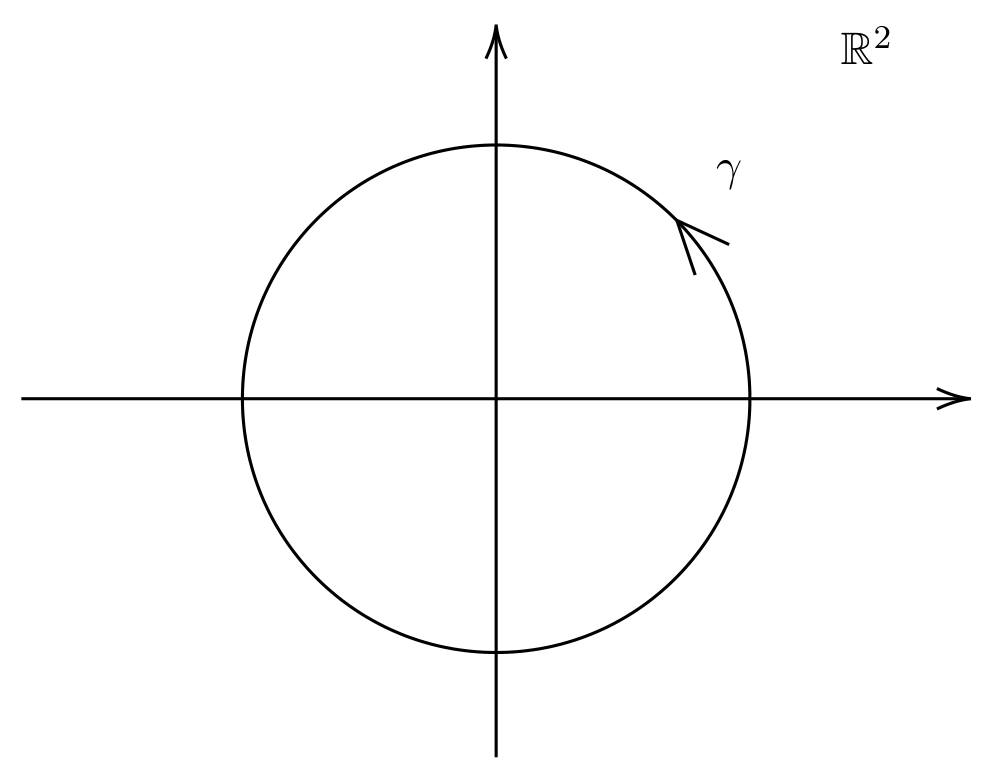
\includegraphics[width=0.46\textwidth]{figures/fig_p259_a.png}
\end{center}
% [图：原书 p.258，图内文字照原样保留]

% [原文 p.259]

复合 $\det^2\circ\gamma$ 是
\[
\det\nolimits^2\circ\gamma:S^1\longrightarrow S^1,\qquad e^{i\theta}\longmapsto e^{2i\theta}.
\]
因此 $\gamma$ 的马斯洛夫指标是
\[
m(\gamma)=2.
\]

\subsection{辛流形}

\begin{definition}{5.1.18}
\emph{辛流形}（symplectic manifold）是指一对 $(M,\omega)$，其中 $M$ 是光滑流形，$\omega$ 是 $M$ 上的光滑 2-形式，满足

① $\omega$ 是闭的：$d\omega=0$；

② $\omega$ 非退化：$\forall p\in M$，
\[
\omega|_p:T_pM\times T_pM\longrightarrow\R
\]
在 $T_pM$ 上给出辛配对。
\end{definition}

在局部坐标 $\{x^i\}$ 下，$\omega$ 可写成
\[
\omega=\frac12\sum_{i,j}\omega_{ij}(x)dx^i\wedge dx^j,
\]
其中 $\omega_{ij}(x)=-\omega_{ji}(x)$。条件 $d\omega=0$ 成为
\[
\partial_i\omega_{jk}+\partial_j\omega_{ki}+\partial_k\omega_{ij}=0,\qquad \forall i,j,k.
\]
非退化条件说的是
\[
\det\big(\omega_{ij}(x)\big)\neq 0,\qquad \forall x.
\]

\begin{definition}{5.1.19}
给定 $M$ 上的光滑函数 $f$，由方程
\[
\iota_{V_f}\omega=df
\]
定义其相联系的\emph{哈密顿向量场}（Hamiltonian vector field）$V_f\in\mathrm{Vect}(M)$。
\end{definition}

具体地，在局部坐标下
\[
V_f=\sum_{i,j}\omega^{ij}\partial_if\frac{\partial}{\partial x^j},
\]
其中 $\{\omega^{ij}\}$ 是 $\{\omega_{ij}\}$ 的逆矩阵，即满足
\[
\sum_k\omega^{ik}\omega_{kj}=\delta^i_j.
\]
事实上，
\[
\sum_{i,j}\omega^{ij}\partial_if\,\iota_{\partial_j}\omega
=\sum_{i,j,k}\omega^{ij}\partial_if\,\omega_{jk}dx^k
=\sum_i\partial_if\,dx^i=df.
\]

% [原文 p.260]

\begin{definition}{5.1.20}
$M$ 上两个光滑函数 $f,g$ 的\emph{泊松括号}（Poisson bracket）定义为
\[
\{f,g\}:=\iota_{V_f}\iota_{V_g}\omega.
\]
利用 $\iota_{V_g}\omega=dg$，它也可以等价地写成
\[
\{f,g\}=\iota_{V_f}(dg)=V_f(g).
\]
在局部坐标下，
\[
\{f,g\}=\sum_{i,j}\omega^{ij}\partial_if\partial_jg.
\]
\end{definition}

\begin{proposition}{5.1.21}
哈密顿向量场保持辛形式 $\omega$，即 $\mathcal{L}_{V_f}\omega=0$。
\end{proposition}

\begin{proof}
利用嘉当公式，有
\[
\mathcal{L}_{V_f}\omega=(d\iota_{V_f}+\iota_{V_f}d)\omega=d(df)+0=0.
\]
\end{proof}

辛形式 $\omega$ 在 $M$ 上诱导体积形式
\[
\frac{1}{n!}\omega^n,\qquad n=\dim M.
\]
作为推论，哈密顿向量场保持体积密度（\emph{刘维尔定理}，Liouville's Theorem）
\[
\mathcal{L}_{V_f}\left(\frac{1}{n!}\omega^n\right)=0.
\]

\begin{proposition}{5.1.22}
$V_{\{f,g\}}=[V_f,V_g]$。
\end{proposition}

\begin{proof}
利用嘉当公式
\[
\begin{aligned}
\iota_{V_{\{f,g\}}}\omega&=d\{f,g\}=d\iota_{V_f}\iota_{V_g}\omega\\
&=\mathcal{L}_{V_f}\iota_{V_g}\omega-\iota_{V_f}d\iota_{V_g}\omega\\
&=\big(\mathcal{L}_{V_f}\iota_{V_g}-\iota_{V_g}\mathcal{L}_{V_f}\big)\omega-\iota_{V_f}ddg\\
&=\iota_{[V_f,V_g]}\omega.
\end{aligned}
\]
由 $\omega$ 的非退化性，
\[
V_{\{f,g\}}=[V_f,V_g].
\]
\end{proof}

\begin{proposition}{5.1.23}
$(C^\infty(M),\{-,-\})$ 定义李代数。映射
\[
C^\infty(M)\longrightarrow\mathrm{Vect}(M),\qquad f\longmapsto V_f
\]
是李代数同态。
\end{proposition}

\begin{proof}
$\{-,-\}$ 显然是斜对称的。只需验证雅可比恒等式：
\[
\{f,\{g,h\}\}+\{g,\{h,f\}\}+\{h,\{f,g\}\}=0.
\]
事实上，利用命题 5.1.22 与 $\{-,-\}$ 的斜对称性，
\begin{align*}
\{\{f,g\},h\}&=V_{\{f,g\}}(h)=[V_f,V_g](h)=V_f(\{g,h\})-V_g(\{f,h\})\\
&=\{f,\{g,h\}\}-\{g,\{f,h\}\}=-\{\{g,h\},f\}-\{\{h,f\},g\}.
\end{align*}
李代数同态性由命题 5.1.22 得到。
\end{proof}

% [原文 p.261]

\begin{example}{5.1.24}（余切丛）
对任意光滑流形 $X$，其余切丛的全空间 $M=T^*X$ 典范地是辛流形。
\end{example}

设 $\{q^i\}$ 是 $X$ 上的局部坐标。标架 $\left\{\frac{\partial}{\partial q^i}\right\}$ 自然给出 $T^*X$ 的纤维上的线性坐标 $\{p_i\}$。于是 $\{q^i,p_i\}$ 构成 $T^*X$ 上的局部坐标。考虑 1-形式
\[
\lambda=\sum_i p_idq^i.
\]
容易验证这个表达式不依赖局部坐标的选取，$\lambda$ 是 $T^*X$ 上整体定义的 1-形式。$\lambda$ 称为\emph{刘维尔 1-形式}（Liouville 1-form）。2-形式
\[
\omega=d\lambda=\sum_i dp_i\wedge dq^i
\]
在 $T^*X$ 上给出辛形式。

\begin{definition}{5.1.25}
设 $(M,\omega)$ 是辛流形。子流形 $L\subset M$ 称为\emph{拉格朗日子流形}（Lagrangian submanifold），若 $\dim L=\frac12\dim M$ 且 $\omega|_L=0$。
\end{definition}

这等价于说：对所有 $p\in L$，切空间 $T_pL$ 是 $(T_pM,\omega|_p)$ 的线性拉格朗日子空间。

设 $M=T^*X$，$\omega$ 是典范辛形式。维数为 $\dim L=\frac12\dim M$ 的子流形 $L\subset M$ 是拉格朗日子流形，当且仅当
\[
\omega|_L=d\lambda|_L=0,
\]
即刘维尔 1-形式在 $L$ 上的限制 $\lambda|_L$ 是闭 1-形式。

我们考虑一个特殊情形。设 $S:X\to T^*X$ 是余切丛的截面。这样的截面等同于指定 $X$ 上的一个 1-形式 $\alpha$，我们把它记为
\[
S_\alpha:X\longrightarrow T^*X.
\]
$S_\alpha$ 的像定义了子流形
\[
L_\alpha:=S_\alpha(X)\subset T^*X.
\]
$S_\alpha$ 的一个好性质是恒等地有
\[
S_\alpha^*(\lambda)=\alpha.
\]
这立刻导致

\begin{proposition}{5.1.26}
$L_\alpha\subset T^*X$ 是拉格朗日子流形，当且仅当 $\alpha$ 是闭 1-形式：$d\alpha=0$。
\end{proposition}

% [原文 p.262]

\begin{center}
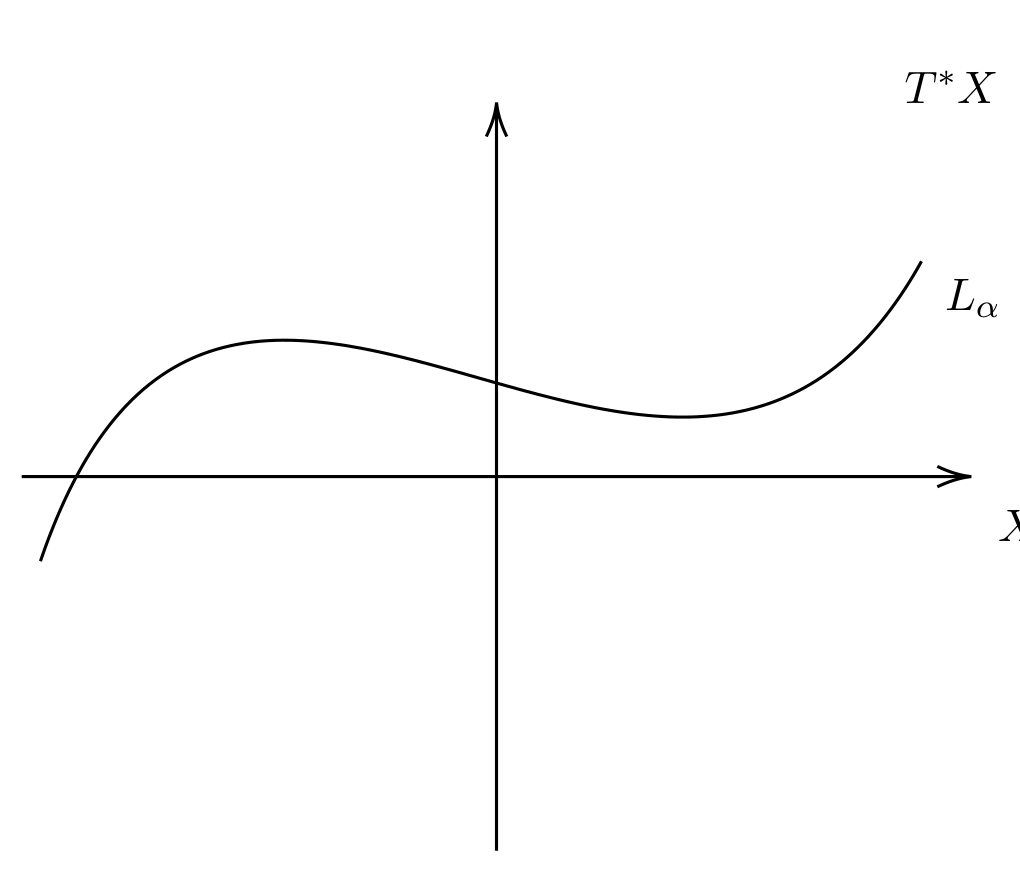
\includegraphics[width=0.52\textwidth]{figures/fig_p263_a.png}
\end{center}
% [图：原书 p.262，图内文字照原样保留]

\begin{definition}{5.1.27}
与闭 1-形式 $\alpha$ 相联系的、形如 $L_\alpha\subset T^*X$ 的拉格朗日子流形，称为 $T^*X$ 的\emph{可投影拉格朗日子流形}（projectable Lagrangian submanifold）。若 $\alpha=df$ 是恰当 1-形式，则称 $L_\alpha$ 为\emph{恰当拉格朗日子流形}（exact Lagrangian）。
\end{definition}

\begin{example}{5.1.28}
对恰当拉格朗日子流形 $L_{df}$，它由方程
\[
p_i=\frac{\partial}{\partial q^i}f(q)
\]
描述。此时称 $f$ 为 $L$ 的\emph{相函数}（phase function）。注意相函数只能确定到相差一个常数。
\end{example}

\begin{example}{5.1.29}
$\R^2=T^*\R$，$\omega=dp\wedge dq$。则 $\R^2$ 中任意曲线都定义拉格朗日子流形。考虑
\[
L=\{p^2+q^2=R^2\}\subset T^*\R.
\]
\end{example}

\begin{center}
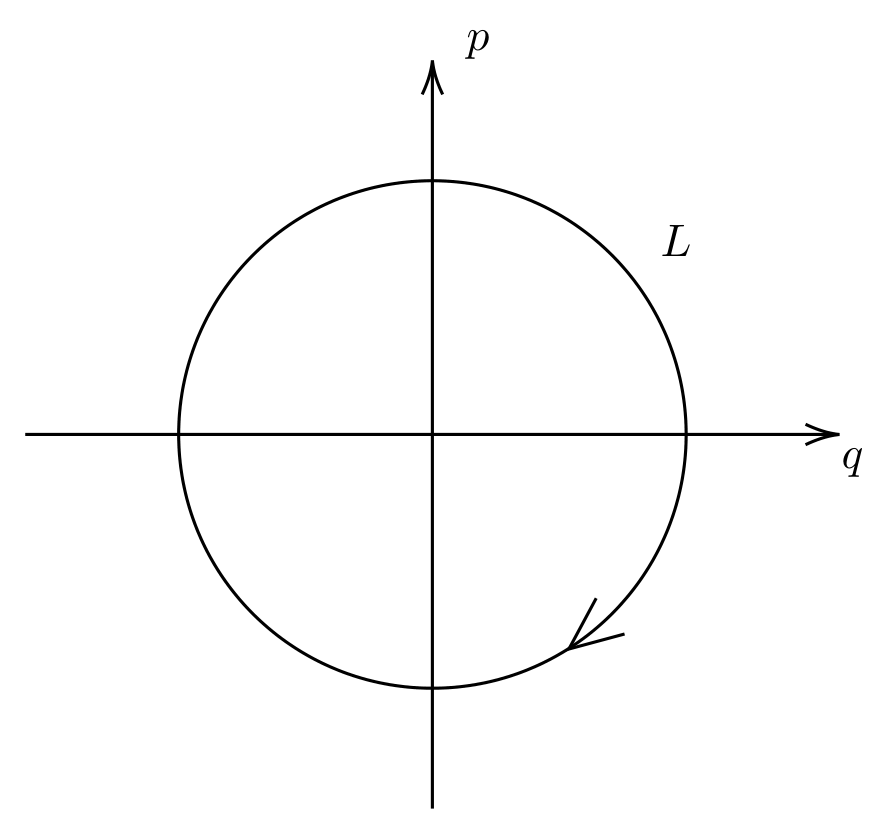
\includegraphics[width=0.42\textwidth]{figures/fig_p263_b.png}
\end{center}
% [图：原书 p.262，图内文字照原样保留]

刘维尔 1-形式 $\lambda=pdq$ 在 $L$ 上的限制是闭的，但不是恰当的，因为
\[
\int_L\lambda=\pm\pi R^2,
\]
其中符号 $\pm$ 取决于 $L$ 的定向。

% [原文 p.263]

\begin{definition}{5.1.30}
微分同胚 $\phi:M\to M$ 称为\emph{辛同胚}（symplectomorphism），若 $\phi$ 保持辛结构，即
\[
\phi^*\omega=\omega.
\]
\end{definition}

\begin{proposition}{5.1.31}
设 $\phi:M\to M$ 是辛同胚，$L\subset M$ 是拉格朗日子流形。则 $\phi(L)$ 也是拉格朗日子流形。
\end{proposition}

\begin{example}{5.1.32}
由哈密顿向量场 $V_f$ 生成的流 $\phi_t:M\to M$ 是辛同胚。事实上，
\[
\frac{d}{dt}(\phi_t^*\omega)=\phi_t^*\big(\mathcal{L}_{V_f}\omega\big)=0
\quad\Longrightarrow\quad
\phi_t^*\omega=\omega,\quad \forall t.
\]
\end{example}

现在把这个例子特殊化到
\[
M=T^*X\qquad\text{与}\qquad f:X\to\R.
\]
把 $f$ 看成 $M$ 上的函数，其相应的哈密顿向量场是
\[
V_f=\sum_i\partial_{q^i}f\frac{\partial}{\partial p_i}.
\]
由 $V_f$ 生成的辛同胚 $\phi_t:T^*X\to T^*X$ 把纤维平移 $tdf$，因此
\[
\phi_1(L_\alpha)=L_{\alpha+df}.
\]
特别地，$\phi_1$ 把零截面变成
\[
\phi_1(L_0)=L_{df}.
\]

\takeaway{本节先在线性层面讲辛向量空间：辛形式、复结构与厄米结构相互对应；再引入拉格朗日子空间与拉格朗日格拉斯曼流形，用 det² 定义马斯洛夫指标；最后把辛结构搬到流形上，给出哈密顿向量场与泊松括号。}

\section{几何半经典量子化}

\subsection{半经典解}

我们考虑在 $\R^n$ 中势 $V(\mathbf{x})$ 里运动的量子粒子。量子哈密顿算子是
\[
\wh{H}=-\frac{\hbar^2}{2m}\nabla^2+V(\mathbf{x}),
\]
薛定谔方程取形式
\[
i\hbar\frac{\partial}{\partial t}\Psi=\wh{H}\Psi.
\]
我们考虑形如（称为\emph{定态}，stationary states）的解
\[
\Psi(\mathbf{x},t)=e^{-iEt/\hbar}\psi(\mathbf{x}).
\]
把它代入薛定谔方程，得到
\[
\wh{H}\psi(\mathbf{x})=E\psi(\mathbf{x}) \tag{$*$}
\]

% [原文 p.264]

于是 $\psi(\mathbf{x})$ 是 $\wh{H}$ 的一个本征态，本征值为 $E$，它解释为能量。方程 ($*$) 称为\emph{定态薛定谔方程}（time-independent Schrödinger equation）。

我们考虑 ($*$) 的形如
\[
\psi=e^{\frac{i}{\hbar}S(\mathbf{x})}a(\mathbf{x},\hbar)
\]
的解。$S(\mathbf{x})$ 称为\emph{相函数}（phase function），$a(\mathbf{x},\hbar)$ 称为\emph{振幅}（amplitude）。注意
\begin{align*}
&\left(-\frac{\hbar^2}{2m}\nabla^2+(V-E)\right)\left(ae^{\frac{i}{\hbar}S}\right)\\
&\quad=\left[a\left(\frac{(\nabla S)^2}{2m}+(V-E)\right)-\frac{\hbar^2}{2m}\nabla^2a-\frac{i\hbar}{2m}\Big(a\nabla^2S+2\nabla S\cdot\nabla a\Big)\right]e^{\frac{i}{\hbar}S}.
\end{align*}
WKB 方法的思想是寻找形如
\[
\psi=e^{\frac{i}{\hbar}S(\mathbf{x})}\big(a_0(\mathbf{x})+a_1(\mathbf{x})\hbar+\cdots\big)
\]
的 $\hbar$-渐近解，即 $a(\mathbf{x},\hbar)$ 具有 $\hbar$-渐近级数
\[
a(\mathbf{x},\hbar)\sim\sum_{k=0}^{\infty}a_k(\mathbf{x})\hbar^k,\qquad a_0(\mathbf{x})\neq0.
\]
把这个 WKB 拟设代入上述方程，得到
\[
\begin{cases}
\dfrac{(\nabla S)^2}{2m}+V=E\\[8pt]
a_0\nabla^2S+2\nabla S\cdot\nabla a_0=0\\[4pt]
a_k\nabla^2S+2\nabla S\cdot\nabla a_k=i\nabla^2a_{k-1},\qquad k\ge1
\end{cases}
\]
近似解
\[
e^{\frac{i}{\hbar}S(\mathbf{x})}a_0(\mathbf{x})
\]
称为\emph{半经典近似}（semi-classical approximation）。

$S$ 的首阶方程可以写成
\[
\mathcal{H}(\mathbf{x},\mathbf{p}=\nabla S)=E \tag{$**$}
\]
这里 $\mathcal{H}(\mathbf{x},\mathbf{p})=\frac{\mathbf{p}^2}{2m}+V(\mathbf{x})$ 是经典哈密顿函数。方程 ($**$) 正是\emph{哈密顿–雅可比方程}（Hamilton–Jacobi equation）。

几何上，$S$ 定义了恰当可投影拉格朗日子流形
\[
L_{dS}\subset T^*\R^n,
\]
而哈密顿–雅可比方程说的是 $\mathcal{H}$ 在 $L_{dS}$ 上是常数（$=E$），即
\[
d\mathcal{H}|_{L_{dS}}=0.
\]
用哈密顿向量场 $V_{\mathcal{H}}$ 表示，这就是
\[
\iota_{V_{\mathcal{H}}}\omega|_{L_{dS}}=0
\]

% [原文 p.265]

即
\[
\omega\big(V_{\mathcal{H}}(p),T_pL_{dS}\big)=0,\qquad \forall p\in L_{dS}.
\]
由于 $L_{dS}$ 是拉格朗日子流形，这等价于
\[
V_{\mathcal{H}}(p)\in T_pL_{dS},\qquad \forall p\in L_{dS},
\]
即哈密顿向量场 $V_{\mathcal{H}}$ 与 $L_{dS}$ 相切。

\begin{center}
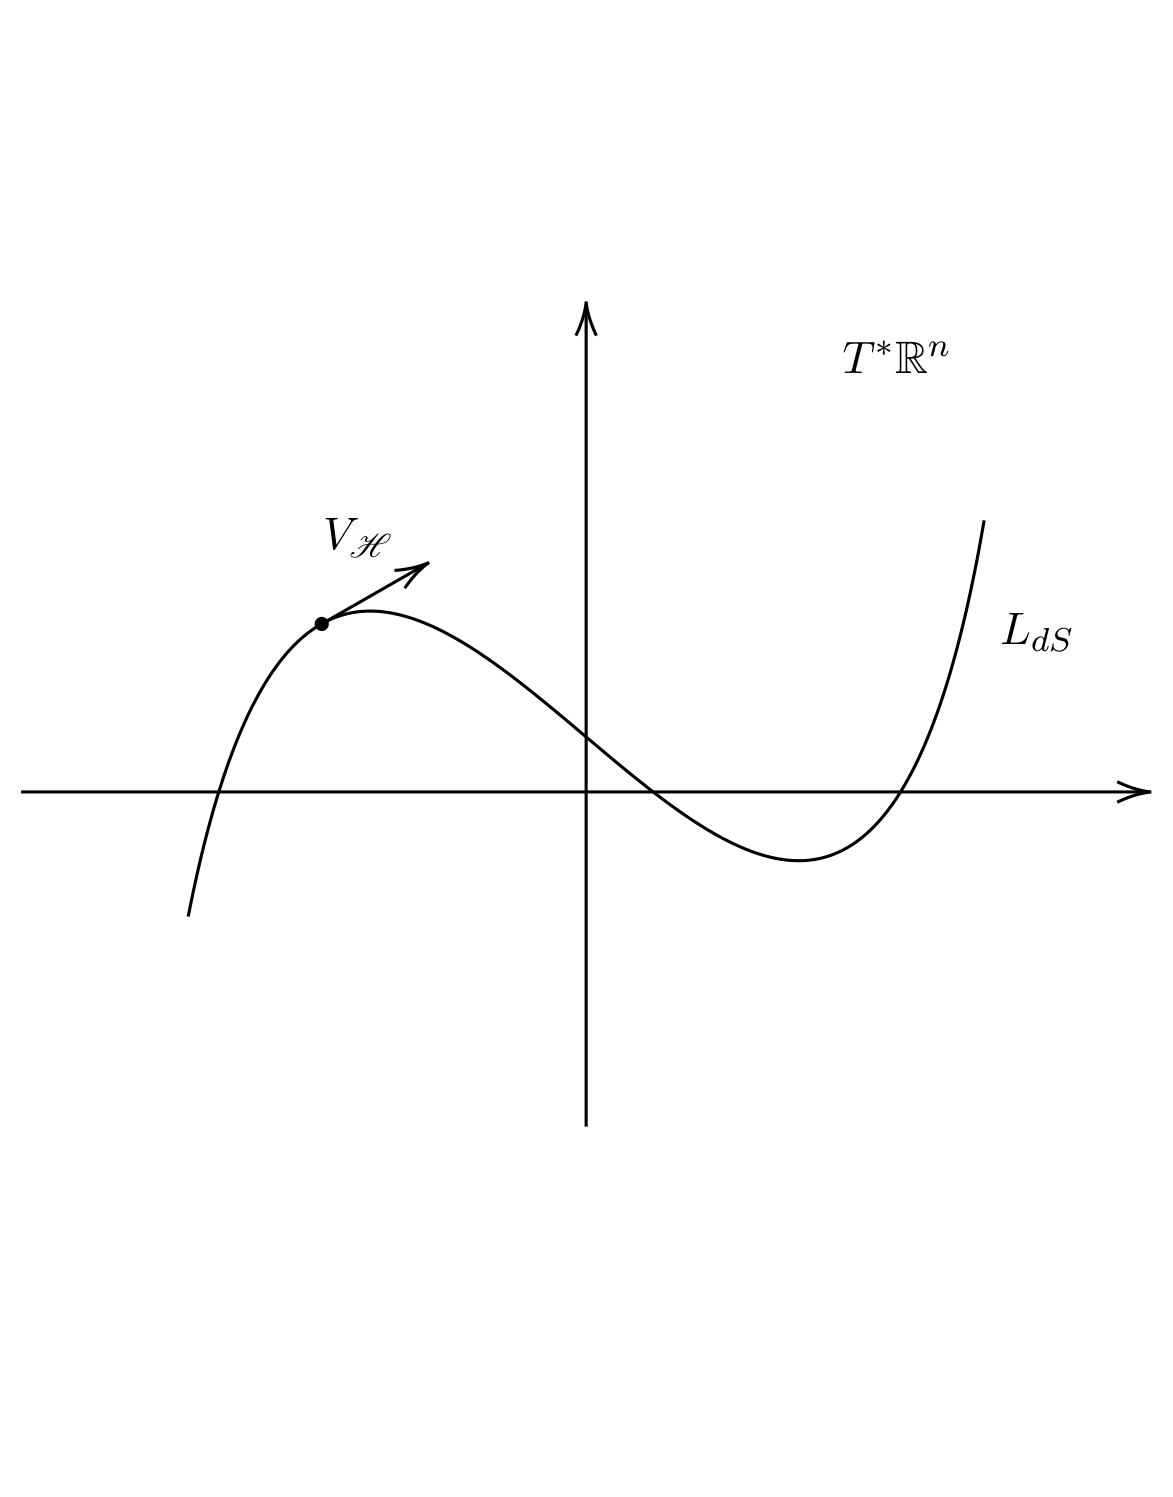
\includegraphics[width=0.52\textwidth]{figures/fig_p266_a.png}
\end{center}
% [图：原书 p.265，图内文字照原样保留]

于是哈密顿–雅可比方程导出这样一张恰当可投影拉格朗日子流形 $L_{dS}$：它以 $S$ 为相函数，且哈密顿向量场 $V_{\mathcal{H}}$ 在 $L_{dS}$ 的每一点都与 $L_{dS}$ 相切。

现在考虑次阶方程
\[
a_0\nabla^2S+2\nabla S\cdot\nabla a_0=0,
\]
它称为\emph{齐次输运方程}（homogeneous transport equation）。它可以写成
\[
\nabla\cdot\big(a_0^2\nabla S\big)=0.
\]
这允许我们把它解释为
\[
\mathcal{L}_{\nabla S}\big(a_0^2|d^nx|\big)=0.
\]

% [原文 p.266]

这里 $|d^nx|=|dx^1\wedge\cdots\wedge dx^n|$ 是 $\R^n$ 上的典范体积密度。$\mathcal{L}_{\nabla S}$ 是关于向量场
\[
\sum_i\partial_iS\frac{\partial}{\partial x^i}
\]
的李导数。

几何上，记 $\pi$ 为微分同胚
\[
\pi:\ L_{dS}\longrightarrow\R^n,\qquad (x^i,p_i=\partial_iS)\longmapsto(x^i).
\]
哈密顿向量场 $V_{\mathcal{H}}$ 是
\[
V_{\mathcal{H}}=\sum_i\left(\frac{\partial\mathcal{H}}{\partial x^i}\frac{\partial}{\partial p_i}-\frac{\partial\mathcal{H}}{\partial p^i}\frac{\partial}{\partial x_i}\right)
=\sum_i\left(\partial_iV\frac{\partial}{\partial p_i}-\frac1mp_i\frac{\partial}{\partial x_i}\right).
\]
注意
\[
\pi_*\big(V_{\mathcal{H}}|_{L_{dS}}\big)=-\frac1m\sum_i\partial_iS\frac{\partial}{\partial x_i}.
\]
于是齐次输运方程成为
\[
\mathcal{L}_{\pi_*(V_{\mathcal{H}}|_{L_{dS}})}\big(a_0^2|d^nx|\big)=0.
\]
由于 $\pi:L_{dS}\to\R^n$ 是微分同胚，我们可以等价地在 $L_{dS}$ 上把它写成
\[
\mathcal{L}_{V_{\mathcal{H}}|_{L_{dS}}}\Big(\pi^*\big(a_0^2|d^nx|\big)\Big)=0.
\]

\subsection{半密度}

回忆流形 $M$ 上的密度线丛 $\mathrm{Dens}_M$ 由这样的截面描述：在局部坐标 $\{x^i\}$ 下它们形如
\[
\rho_x(x)|d^nx|,\qquad \rho_x(x)\ \text{是光滑函数}.
\]
在坐标变换 $\{x^i\}\to\{y^i\}$ 下，两个坐标中的 $\rho_x$ 与 $\rho_y$ 由
\[
\rho_x=\rho_y\left|\det\left(\frac{\partial y}{\partial x}\right)\right|
\]
相联系。这里 $\left(\frac{\partial y}{\partial x}\right)=\left(\frac{\partial y^i}{\partial x^j}\right)$ 是雅可比矩阵。换言之，密度线丛的转移函数是 $\left|\det\left(\frac{\partial y}{\partial x}\right)\right|$。不变地，我们可以把它写成
\[
\rho_x|d^nx|=\rho_y|d^ny|.
\]
这一性质使我们可以在流形上对密度积分
\[
\int_M:\Gamma(M,\mathrm{Dens}_M)\longrightarrow\R,\qquad \rho\longmapsto\int_M\rho
\]

% [原文 p.267]

\begin{remark}{5.2.1}
若 $M$ 可定向，选取一个定向，便可把二者等同：
\[
\mathrm{Dens}_M\simeq\Lambda^nT^*M,\qquad n=\dim M,
\]
于是 $\mathrm{Dens}_M$ 的截面成为 $n$-形式。当 $M$ 不可定向时，这两个丛是不同的。
\end{remark}

类似地，对任意 $\alpha>0$，可以定义 $\alpha$-密度线丛 $\mathrm{Dens}_M^\alpha$，其转移函数由
\[
\left|\det\left(\frac{\partial y}{\partial x}\right)\right|^\alpha
\]
给出。不变地，$\alpha$-密度局部可写成
\[
\rho_x|d^nx|^\alpha.
\]
转移函数说明：在坐标变换 $\{x^i\}\to\{y^i\}$ 下，有
\[
\rho_x|d^nx|^\alpha=\rho_y|d^ny|^\alpha.
\]

回到半经典解，更好的做法是把 $a_0(\mathbf{x})$ 看成半密度
\[
a_0|d^nx|^{1/2}.
\]
在微分同胚 $\pi:L_{dS}\to\R^n$ 下，它在 $L_{dS}$ 上给出半密度 $\pi^*\big(a_0|d^nx|^{1/2}\big)$。于是齐次输运方程可以写成
\[
\mathcal{L}_{V_{\mathcal{H}}|_{L_{dS}}}\left(\pi^*\Big(a_0\,|d^nx|^{1/2}\Big)\right)=0.
\]
总之，我们得到如下描述：定态薛定谔方程的半经典解等价于如下几何数据：

① 一张恰当可投影拉格朗日子流形 $L$，它落在哈密顿函数 $\mathcal{H}$ 的一个水平集里（等价地，$V_{\mathcal{H}}$ 与 $L$ 相切）；

② $L$ 上的一个半密度 $\Omega$，它在哈密顿向量场 $V_{\mathcal{H}}$ 下不变。

给定这样的数据，记 $S$ 为 $L$ 的相函数（确定到相差一个常数）。设
\[
s:\R^n\longrightarrow L,\qquad (x^i)\longmapsto(x^i,p_i=\partial_iS)
\]
为截面映射所给的微分同胚。设
\[
s^*\Omega=a_0(x)|d^nx|^{1/2}
\]
是它在 $\R^n$ 上表示的相应半密度。则
\[
e^{\frac{i}{\hbar}S(x)}a_0(x)
\]
给出一个半经典解。

这样的几何描述有一个直接的好处：$L$ 可以是一般的拉格朗日子流形，而不必是恰当可投影的。对落在 $\mathcal{H}$ 的水平集中的这种 $L$，$V_{\mathcal{H}}$-不变半密度的概念仍然良定义。这就引出了我们下面要讨论的几何半经典态。

% [原文 p.268]

\subsection{马斯洛夫修正}

现在我们考虑拉格朗日子流形 $L\subset T^*\R^n$ 上的量子化，这里 $L$ 不必可投影。$L$ 上使
\[
\pi:L\longrightarrow\R^n
\]
不能成为局部微分同胚的点称为\emph{焦散}（caustics）。

\begin{example}{5.2.2}
考虑一维谐振子
\[
\mathcal{H}=\frac{p^2}{2m}+\frac12kx^2.
\]
水平集 $\mathcal{H}=E>0$ 是拉格朗日子流形
\[
L=\{(x,p)\mid \mathcal{H}(x,p)=E\}.
\]
\end{example}

\begin{center}
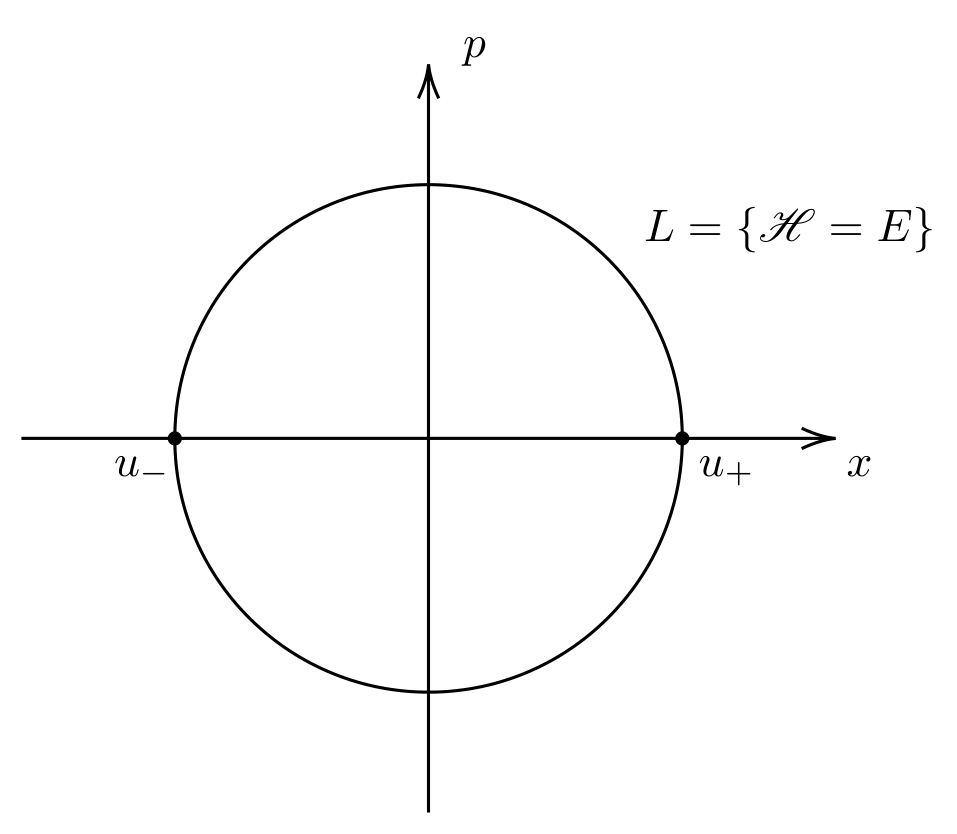
\includegraphics[width=0.40\textwidth]{figures/fig_p269_a.png}
\end{center}
% [图：原书 p.268，图内文字照原样保留]

$L$ 有两个焦散，由
\[
u_\pm=\left(\pm\sqrt{\frac{2E}{k}},0\right)
\]
给出。

焦散不是 $L$ 的奇点。它们其实反映了我们从位形空间选取坐标 $x$ 的方式。事实上，若考虑向 $p$-坐标的投影
\[
\pi_P:L\longrightarrow\R,\qquad (x,p)\longmapsto p,
\]
则 $\pi_P$ 在 $u_\pm$ 附近是局部微分同胚。这提示我们可以在拉格朗日子流形附近的局部取适当坐标做量子化，再粘合起来。这正是马斯洛夫的手法。

受可投影情形的启发，我们如下定义几何半经典态。

\begin{definition}{5.2.3}
\emph{几何半经典定态}（geometric semi-classical stationary state）是指一对 $(L,\Omega)$，其中

① $L\subset T^*X$ 是拉格朗日子流形，落在哈密顿函数 $\mathcal{H}$ 的一个水平集里；

② $\Omega$ 是 $L$ 上的半密度，在哈密顿向量场 $V_{\mathcal{H}}$ 下不变。
\end{definition}

% [原文 p.269]

下面我们来考察，如何把半经典解
\[
e^{\frac{i}{\hbar}S}a\,|d^nx|^{1/2}
\]
的类比实现在几何半经典态 $(L,\Omega)$ 上。

当 $L=L_{dS}$ 是恰当可投影时，相函数 $S$（视为 $L$ 上的函数）是
\[
S=\int\lambda
\]
确定到相差一个常数。这里 $\lambda=\sum_ip_idx^i$ 是刘维尔 1-形式。这等同于说
\[
\lambda|_L=dS.
\]
对一般的拉格朗日子流形 $L$，我们有
\[
\lambda|_L\ \text{是闭的},
\]
但可能不是恰当的。尽管如此，我们仍希望用
\[
e^{\frac{i}{\hbar}\int_{z_0}^{z}\lambda},\qquad z\in L
\]
来定义相位因子。这里 $z_0\in L$ 是某个参考基点。积分 $\int_{z_0}^z\lambda$ 是多值的，依赖于从 $z_0$ 到 $z$ 的积分路径。从 $z_0$ 到 $z$ 的两条路径相差一个闭链 $\gamma$，相应的积分 $\int_{z_0}^z\lambda$ 相差
\[
\oint_\gamma\lambda.
\]
注意，由于 $\lambda$ 在 $L$ 上是闭的，闭路积分 $\oint_\gamma\lambda$ 只依赖 $\gamma$ 在 $H_1(L)$ 中的拓扑类。

\begin{center}
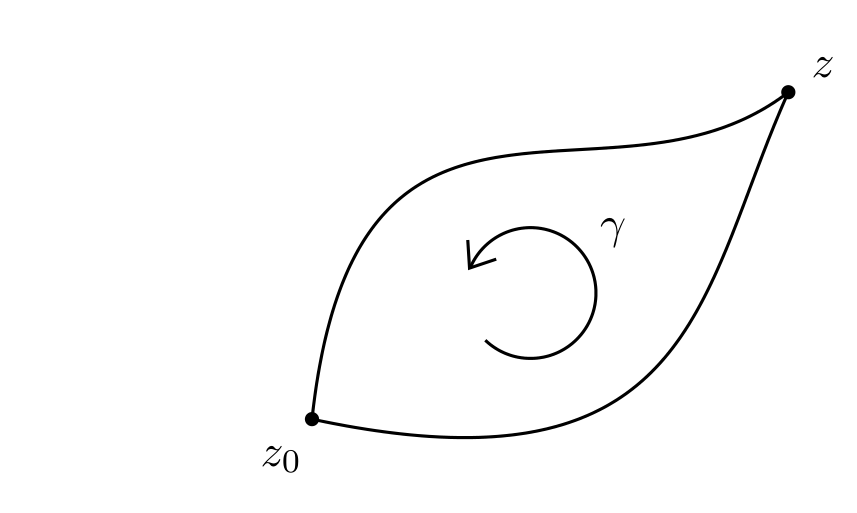
\includegraphics[width=0.40\textwidth]{figures/fig_p270_c.png}
\end{center}
% [图：原书 p.269，图内文字照原样保留]

因此，若对一切 $\gamma\in H_1(L)$ 都有 $\frac1\hbar\oint_\gamma\lambda\in2\pi\Z$，则 $e^{\frac{i}{\hbar}\int_{z_0}^z\lambda}$ 会是 $L$ 上良定义的函数。这提示如下整性条件（\emph{玻尔–索末菲量子化条件}，Bohr–Sommerfeld quantization condition）
\[
\frac{1}{2\pi\hbar}\oint_\gamma\lambda\in\Z
\]
对所有 $L$ 上的闭 1-链 $\gamma$ 成立。当 $L$ 可投影时，这会被满足。然而当焦散出现时，还有进一步的修正，称为\emph{马斯洛夫修正}（Maslov correction）。

% [原文 p.270]

问题出在半经典解中的半密度部分。在可投影的情形，$L$ 可以通过投影与 $\R^n$ 等同，我们可以统一地取平方根 $|d^nx|^{1/2}$，并写成
\[
\pi_*\Omega=a(x)\,|d^nx|^{1/2}.
\]
这时 $e^{\frac{i}{\hbar}S}a$ 就给出半经典解。一般情形下，我们需要弄清如何在 $L$ 上一致地取体积密度的平方根。

设 $L$ 可定向，并把密度线丛与
\[
\mathrm{Dens}_L\simeq\Lambda^nT^*L
\]
等同，后者是 $\Lambda^nT_*L$ 的对偶。在每一点 $z\in L$，切平面
\[
T_zL\subset T_z(T^*\R^n)=\R^{2n}
\]
给出一个拉格朗日线性子空间，即
\[
T_zL\in\mathcal{L}(\R^{2n}),
\]
它是拉格朗日格拉斯曼流形的一个元素。

回忆我们可以等同
\[
\mathcal{L}(\R^{2n})\simeq \mathrm{U}(n)/\mathrm{O}(n),
\]
连同
\[
\mathcal{L}(\R^{2n})\xrightarrow{\ \det^2\ }S^1,
\]
这诱导出同构
\[
\pi_1\big(\mathcal{L}(\R^{2n})\big)\simeq\pi_1(S^1).
\]
具体地，我们取标准的复结构来等同
\[
\R^{2n}\overset{J}{\simeq}\C^n=\R^n\oplus J\R^n,
\]
其中 $\R^n=\Span\{e_1,\cdots,e_n\}$，$J\R^n=\Span\{f_1,\cdots,f_n\}$。于是 $\{e_1,\cdots,e_n\}$ 给出 $\C^n=\R^{2n}$ 的一组 $\C$-基。对一个拉格朗日子空间 $L_0$，我们取它的一组正交归一基 $\{c_1,\cdots,c_n\}$。则
\[
\det{}^2(L_0)=\left[\frac{c_1\wedge_\C\cdots\wedge_\C c_n}{e_1\wedge_\C\cdots\wedge_\C e_n}\right]^2\in S^1.
\]
这里 $\wedge_\C$ 是 $\C^n$ 上的 $\C$-线性楔积。这使我们能定义一个映射
\[
\varphi:\ \Big(\Lambda^nL_0^{\vee}\Big)^2-\{0\}\longrightarrow\C^*,\qquad (\alpha)^2\longmapsto re^{-i\theta},
\]
其中
\[
r=\big(\alpha(c_1,\cdots,c_n)\big)^2,\qquad e^{i\theta}=\det{}^2(L_0).
\]
这个映射 $\varphi$ 不依赖 $L_0$ 的基 $\{c_1,\cdots,c_n\}$ 的选取。

% [原文 p.271]

我们把这个构造用到拉格朗日子流形 $L\subset T^*\R^n$ 上，得到映射
\[
\varphi:\ \Big(\Lambda^nT^*L\Big)^2-\{\text{零截面}\}\longrightarrow\C^*.
\]
映射 $\varphi$ 可以看成描述 $L$ 上 2-密度相对于 $\R^n$ 上一个固定参考 2-密度的几何变化。我们把 $\varphi$ 的 $S^1$-相位部分写成
\[
\Theta=\frac{\varphi}{|\varphi|}:\ \Big(\Lambda^nT^*L\Big)^2-\{\text{零截面}\}\longrightarrow S^1.
\]
$\Theta$ 表示 2-密度沿 $L$ 的几何相位变化。

现在考虑 $L$ 上的半密度 $\Omega$。要描述半经典解，我们需要把 $\Omega$ 与位形空间 $\R^n$ 上的标准半密度作比较。在焦散附近，相对于雅可比的直接比较会发散；为绕过这一困难，我们采用上面的几何比较 $\varphi$。按构造，我们可以把 $\varphi$ 看成 2-密度相对于某固定点处参考 2-密度的连续参数化。对 $L$ 上的半密度 $\Omega$，$\Omega^4$ 是一个 2-密度。于是我们可以用
\[
\varphi(\Omega^4)^{1/4}=\Theta^{1/4}\big|\varphi(\Omega^4)\big|^{1/4}
\]
来参数化半密度 $\Omega$。

然而 $\Theta^{1/4}$ 在 $L$ 上是多值的。当它绕 $L$ 中的闭路 $\gamma$ 走一圈时，$\Theta^{1/4}$ 改变
\[
e^{-\frac i4(2\pi m(\gamma))},
\]
这里 $m(\gamma)$ 是马斯洛夫指标。

下面我们把半密度与相函数结合起来，考虑几何半经典波
\[
e^{\frac i\hbar\int^z\lambda}\,\Theta^{1/4}\big|\varphi(\Omega^4)\big|^{1/4}.
\]
它的多值性现在体现为沿闭 1-链 $\gamma$ 走一圈时相位因子的改变
\[
e^{\frac i\hbar\oint_\gamma\lambda-\frac i4(2\pi m(\gamma))}.
\]
因此，上述几何半经典波在 $L$ 上整体定义，当且仅当
\[
\frac{1}{2\pi\hbar}\oint_\gamma\lambda-\frac14m(\gamma)\in\Z
\]
对 $L$ 上每条闭 1-链 $\gamma$ 成立。这一规则就是\emph{凯勒–马斯洛夫}量子化条件（Keller–Maslov quantization condition）。因子 $\frac14m(\gamma)$ 就是\emph{马斯洛夫修正}。在物理学文献中，它被称为\emph{爱因斯坦–布里渊–凯勒}（Einstein–Brillouin–Keller，EBK）半经典量子化条件，借助马斯洛夫指标改进了玻尔–索末菲规则。

\begin{example}{5.2.4}
考虑一维谐振子
\[
\mathcal{H}=\frac{p^2}{2m}+\frac12kx^2.
\]
水平集
\[
C=\{\mathcal{H}(x,p)=E\}
\]
是一张拉格朗日子流形。
\end{example}

% [块界：本块末句「The level set $C=\{\mathcal{H}(x,p)=E\}$ is a Lagrangian submanifold.」起于 PDF p.272（原书 p.271）末、谓语在 PDF p.273（原书 p.272）首，已按下一页页图补全；ch05b 由 tr07 从原书 p.272 的 “We have …” 起译，勿重复本句。§5.2 在本块起头、未在本块收尾。]








